\documentclass[10pt,hyperref={pdfpagemode=FullScreen},aspectratio=169]{beamer}

\usetheme[progressbar=frametitle]{metropolis}
\usepackage{appendixnumberbeamer}
\usepackage{lipsum}
\usepackage{amsmath}
\usepackage{amssymb}
\usepackage{booktabs}
\usepackage{siunitx}
\usepackage[scale=2]{ccicons}
\usepackage{pgfplots}
\usepgfplotslibrary{dateplot}
\usepackage{tikz}
\usetikzlibrary{positioning, shapes.geometric}
\pgfplotsset{compat=newest} % Allows to place the legend below plot
\usepgfplotslibrary{units} % Allows to enter the units nicely
\usepackage{circuitikz}
\usetikzlibrary{shapes,arrows}
\usepackage{dirtytalk}
\usepackage{xspace}




% Bibliography
\usepackage[
    backend=biber,
    style=ieee,
    natbib=true,
    url=false, 
    doi=true,
    eprint=false
]{biblatex}
%\addbibresource{references.bib}


\newcommand{\themename}{\textbf{\textsc{metropolis}}\xspace}
\newcommand{\universidade}{Universidade de Brasília}
\newcommand{\doctitle}{Introduction to AASP}

\definecolor{mpigreen}{HTML}{007977}
\setbeamercolor{frametitle}{bg=mpigreen}

\title{\doctitle}

\author{Daniel Araújo}
\institute{\universidade}
\titlegraphic{\hfill
\includegraphics[height=1.5cm]{../logo}}

\title{Modulação AM}

\author{Prof. Daniel Costa Araújo}

\usepackage{graphicx}
\usepackage{subfigure}
\usepackage{verbatim}
\begin{document}


\frame{\titlepage}


\section{Introdução}

\begin{frame}{O que é modulação?}
  \begin{itemize}
      \item A modulação é o processo de variação de um ou mais parâmetros de uma onda portadora em função do sinal de informação.
      \item Parâmetros comuns a serem modulados:
      \begin{itemize}
          \item Amplitude
          \item Frequência
          \item Fase
      \end{itemize}
      \item A modulação permite transmitir informações a longas distâncias e alocar vários sinais no espectro eletromagnético.
  \end{itemize}
  \end{frame}

\begin{frame}
 
    \frametitle{Conceito}

\begin{block}{Vantagens}

    \begin{itemize}
        \item Conversão de frequência
        \item Redução do tamanho das antenas
        \item Acomodar diferentes sinais 
    \end{itemize}
    
\end{block}


\begin{block}{Tipos de Modulação}
    \begin{itemize}
        \item Double side-band supressed carrier (DSB-SC)
        \item DSB full carrier (DSB-FC)
        \item Single Side Band (SSB)
        \item Vestigial Side Band (VSB)
    \end{itemize}
    
\end{block}
\end{frame}

\section{DSB-SC}

\begin{frame}
    \frametitle{Mensagem} 

    \begin{block}{Definição}
        É a informação que será transmitida pelo canal de comunicação \\        
    \end{block}
    \begin{block}{Exemplo}
        $$ 
        m(t) = A_m cos(2\pi f_m t)
        $$
    \end{block}
    \begin{figure}[!h]
        
\includegraphics[width=0.7\textwidth]{Fig/th-1488438850.jpg}
    \end{figure}
\end{frame}


\begin{frame}
    \frametitle{Exemplo de sinal de Mensagem}

    \begin{figure}[h!]
        \begin{center}
          \begin{tikzpicture}
            \begin{axis}[
                width=0.6\textwidth, % Scale the plot to \linewidth
                grid=major, % Display a grid
                grid style={dashed,gray!30}, % Set the style
                xlabel= Tempo, % Set the labels
                ylabel= Amplitude,
                x unit=\si{\second}, % Set the respective units
                y unit=\si{\volt},
                legend style={at={(1,1)},anchor=north west}, % Put the legend below the plot
                x tick label style={rotate=90,anchor=east} % Display labels sideways
              ]
              \addplot+ [no marks]
              % add a plot from table; you select the columns by using the actual name in
              % the .csv file (on top)
              table[x=Tempo,y=Amplitude(V),col sep=comma] {Fig/sinal_mensagem.csv}; 
              \legend{Sinal mensagem.}
            \end{axis}
          \end{tikzpicture}
          \caption{Sinal mensagem.}
        \end{center}
      \end{figure}
    
\end{frame}


\begin{frame}
    \frametitle{Definição de Portadora}
\begin{itemize}
    \item  Para transmitir a informação, considere um função senoidal  
      
  $$ 
  c(t) = A_c cos(2\pi f_c t + \phi _c)
  $$
    
  \item O sinal modulado na saída do modulador AM-DSB é  

  $$
     s(t) = m(t)*c(t)
  $$

\end{itemize}

\end{frame}

\begin{frame}
    \frametitle{Exemplo de sinal modulado}

    \begin{figure}[h!]
        \begin{center}
          \begin{tikzpicture}
            \begin{axis}[
                width=0.6\textwidth, % Scale the plot to \linewidth
                grid=major, % Display a grid
                grid style={dashed,gray!30}, % Set the style
                xlabel= Tempo, % Set the labels
                ylabel= Amplitude,
                x unit=\si{\second}, % Set the respective units
                y unit=\si{\volt},
                legend style={at={(1,1)},anchor=north west}, % Put the legend below the plot
                x tick label style={rotate=90,anchor=east} % Display labels sideways
              ]
              \addplot+ [no marks]
              % add a plot from table; you select the columns by using the actual name in
              % the .csv file (on top)
              table[x=Tempo,y=Amplitude(V),col sep=comma] {Fig/sinal_am_dsbsc.csv}; 


              \addplot+ [no marks,dashed, red]
              % add a plot from table; you select the columns by using the actual name in
              % the .csv file (on top)
              table[x=Tempo,y=Mensagem,col sep=comma] {Fig/sinal_am_dsbsc.csv}; 
              
              
              \legend{Sinal Modulado, Sinal Mensagem}


            \end{axis}
          \end{tikzpicture}
          \caption{Sinal Modulado.}
        \end{center}
      \end{figure}
    
\end{frame}


\begin{frame}
    \frametitle{Análise em Frequência}

    Considere o sinal transmitido no tempo:
$$
 u(t) = m(t)\cos(2\pi f_c t) 
$$
Utilizando a transformada de Fourier:
\begin{align}
    U(f) &= M(f) \circ C(f) \nonumber \\
      &= M(f) \circ \frac{1}{2}(\delta (f - f_c) + \delta (f - f_c))  \nonumber \\
      &=  M(f) \circ \frac{1}{2}\delta(f - f_c) +  M(f) \circ \frac{1}{2}\delta(f - f_c) \nonumber \\ 
      &= \frac{1}{2} M(f - f_c) + \frac{1}{2}M(f + f_c)
\end{align}
 

\begin{block}{IMPORTANTE}
    A modualação AM desloca o espectro da mensagem para a frequência da portadora.   
\end{block} 

\end{frame}

\begin{frame}
  \frametitle{Gráfico em Frequência}
 

  \begin{figure}[h!]
    \begin{center}
      \begin{tikzpicture}
        \begin{axis}[
            width=0.5\textwidth, % Scale the plot to \linewidth
            grid = major, % Display a grid
            grid style={dashed,gray!30}, % Set the style
            xlabel= Frequência, % Set the labels
            ylabel= Amplitude,
            ymin=0, ymax=0.25,
            x unit=\si{\hertz}, % Set the respective units
            y unit=\si{\volt},
            legend style={at={(1,1)},anchor=north west}, % Put the legend below the plot
            %x tick label style={rotate=90,anchor=east} % Display labels sideways
          ]
          
          \addplot+ [no marks]
          table[x=Frequencia,y=Amplitude(V),col sep=comma] {Fig/sinal_freq_am_dsbsc.csv}; 

          \legend{Sinal Modulado}
        \end{axis}
      \end{tikzpicture}
      \caption{Representação em frequência do sinal modulador.}
    \end{center}
  \end{figure}

\end{frame}

\begin{frame}
  \frametitle{ Potência do sinal transmitido}
\begin{block}{Cálculo da potência}
  \begin{align}
    P_n & = \lim _ {T \rightarrow \infty} \int _{-T/2}^{T/2} u^2(t) dt \nonumber \\
       &=  \lim _ {T \rightarrow \infty} \int _{-T/2}^{T/2} A_c^2 m^2(t)\cos^2(2\pi f_c t)  dt \nonumber \\
       &= \frac{A_c^2}{2} \lim _ {T \rightarrow \infty} \int _{-T/2}^{T/2}  m^2(t)[1 + \cos(4\pi f_c t)]dt \nonumber \\
       &=  \frac{A_c^2}{2} P_m
   \end{align}
  
  em que, $P_n = \lim _ {T \rightarrow \infty} \int _{-T/2}^{T/2} m^2(t)dt$
\end{block}
 
\end{frame}


\begin{frame}
  \frametitle{ Demodualação de sinais DSB-SC}

Para simplificar nossa análise considere o sinal recebido igual ao sinal transmitido 
\begin{align}
  r(t) &= u(t) \nonumber \\
       &= m(t)\cos(2\pi f_c t) \nonumber 
\end{align}
Como primeiro passo, utilizamos um oscilador local para realocar a mensagem em sua frequência original.
\begin{align}
  r(t)\cos(2\pi f_c t + \phi) & =  m(t)\cos(2\pi f_c t) \cos(2\pi f_c t + \phi)  \nonumber  \\ 
   & =  \frac{1}{2}m(t)[\cos(\phi) + \cos(4\pi f_c t + \phi)] \nonumber 
\end{align}

\begin{block}{OBSERVAÇÕES:}
  \begin{itemize}
    \item   Presença de componente de alta-frequência
    \item Necessário remover $\phi$ indica sincronização necessária
    \item  Se $\phi = \frac{\pi}{2}$ a informação estará completamente perdida.
  \end{itemize}
\end{block}

\end{frame}


\begin{frame}
  \frametitle{Gráfico em Frequência}
 

  \begin{figure}[h!]
    \begin{center}
      \begin{tikzpicture}
        \begin{axis}[
            width=0.5\textwidth, % Scale the plot to \linewidth
            grid = major, % Display a grid
            grid style={dashed,gray!30}, % Set the style
            xlabel= Frequência, % Set the labels
            ylabel= Amplitude,
            ymin=0, ymax=0.5,
            x unit=\si{\hertz}, % Set the respective units
            y unit=\si{\volt},
            legend style={at={(1,1)},anchor=north west}, % Put the legend below the plot
            %x tick label style={rotate=90,anchor=east} % Display labels sideways
          ]
          
          \addplot+ [no marks]
          table[x=Frequencia,y=Amplitude2(V),col sep=comma] {Fig/sinal_freq_am_dsbsc.csv}; 

          \addplot+ [no marks,dashed,red]
          table[x=Frequencia,y=Amplitude(V),col sep=comma] {Fig/sinal_freq_am_dsbsc.csv}; 


          \legend{Sinal após o mixer, Sinal modulado}
        \end{axis}
      \end{tikzpicture}
      \caption{Representação em frequência na entrada no demodulador.}
    \end{center}
  \end{figure}

\end{frame}


\begin{frame}
  \frametitle{Utilização de um Filtro Passa-baixa}

  \begin{figure}[!t]
    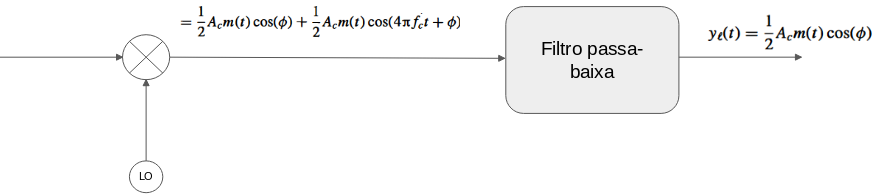
\includegraphics[width = 0.85\textwidth ]{Fig/rx_dsb.png}
    \caption{Filtragem das altas frequências}
  \end{figure}

  \begin{block}{Comentários}
    \begin{itemize}
     \item Um filtro passa-baixa é um componente eletrônico que permite a passagem de sinais com frequências abaixo de um limite específico, chamado de frequência de corte, e atenua os sinais com frequências acima desse limite. 
     \item É usado para remover ruídos e interferências de alta frequência indesejadas que ainda possam estar presentes no sinal. Isso melhora a qualidade do som reproduzido pelos alto-falantes ou fones de ouvido.
    \end{itemize}
  
  \end{block}


\end{frame}

\begin{frame}
  \frametitle{Sinal Demodulado}

  \begin{figure}[h!]
    \begin{center}
      \begin{tikzpicture}
        \begin{axis}[
            width=0.5\textwidth, % Scale the plot to \linewidth
            grid = major, % Display a grid
            grid style={dashed,gray!30}, % Set the style
            xlabel= Tempo, % Set the labels
            ylabel= Amplitude,
            ymin=-1, ymax=1,
            x unit=\si{\second}, % Set the respective units
            y unit=\si{\volt},
            legend style={at={(1,1)},anchor=north west} % Put the legend below the plot
            %x tick label style={rotate=90,anchor=east} % Display labels sideways
          ]
          
          \addplot+ [no marks]
          table[x=Tempo,y=Mensagem,col sep=comma] {Fig/sinal_estimado.csv}; 

          \addplot+ [no marks,black]
          table[x=Tempo,y=Mensagem_Estimada,col sep=comma] {Fig/sinal_estimado.csv}; 


          \legend{Mensagem, Mensagem estimada}
        \end{axis}
      \end{tikzpicture}
      \caption{Comparação entre a mensagem estimada e mensagem real.}
    \end{center}
  \end{figure}

\end{frame}


\section{AM Convencional}

\begin{frame}{Princípios da AM Convencional}
  
  \begin{itemize}
      \item Na AM convencional, a onda portadora e as duas bandas laterais (superior e inferior) são transmitidas.
      \item As bandas laterais são simétricas em relação à frequência da portadora e contêm a mesma informação.
      \item A largura de banda total de um sinal AM convencional é o dobro da largura de banda do sinal de informação.
  \end{itemize}
\end{frame}
 
\begin{frame}
  \begin{block}{Vantagens}
  \begin{itemize}
      \item Simplicidade: A modulação e a demodulação AM são relativamente simples de implementar.
      \item Compatibilidade: A AM convencional é compatível com a maioria dos rádios de ondas médias e curtas disponíveis no mercado.
  \end{itemize}
  \end{block}
  
  \begin{block}{Desvantagens}
  \begin{itemize}
      \item Largura de banda: A AM convencional é ineficiente em termos de largura de banda, pois transmite duas bandas laterais idênticas.
      \item Suscetibilidade a ruído: A AM convencional é mais suscetível a ruído e interferências, resultando em uma qualidade de áudio inferior em comparação com outras técnicas, como a modulação em frequência (FM) ou a modulação de banda lateral única (SSB).
      \item Eficiência energética: A AM convencional consome mais energia durante a transmissão, pois a onda portadora também é transmitida junto com as bandas laterais.
  \end{itemize}
  \end{block}

\end{frame}

\begin{frame}
  \frametitle{Sinal Modulado}

  \begin{columns}[T] % A opção "T" alinha o conteúdo das colunas pelo topo
    \begin{column}{0.5\textwidth}
      \begin{figure}[h!]
        \begin{center}
          \begin{tikzpicture}
            \begin{axis}[
                width=0.85\textwidth, % Scale the plot to \linewidth
                grid = major, % Display a grid
                grid style={dashed,gray!30}, % Set the style
                xlabel= Tempo, % Set the labels
                ylabel= Amplitude,
                ymin=-1.5, ymax=1.5,
                x unit=\si{\second}, % Set the respective units
                y unit=\si{\volt},
                legend style={at={(0,1.5)},anchor=north west} % Put the legend below the plot
                %x tick label style={rotate=90,anchor=east} % Display labels sideways
              ]
              
              \addplot+ [no marks]
              table[x=Tempo,y=Sinal,col sep=comma] {Fig/sinal_am_convencional.csv}; 
    
              \addplot+ [no marks,dashed,red]
              table[x=Tempo,y=Mensagem,col sep=comma] {Fig/sinal_am_convencional.csv}; 
    
    
              \legend{Sinal AM Convencional, Mensagem}
            \end{axis}
          \end{tikzpicture}
          \caption{Sinal AM convecional}
        \end{center}
      \end{figure}
    \end{column}
    \begin{column}{0.5\textwidth}
      \begin{block}{Equação}
        $$
        s(t)  = A_c \left(1 + \alpha m(t)\right) \cos(2\pi f_c t)
        $$
        \begin{itemize}
          \item $\alpha$ é índice de Modulação
          \item Sinal esta no envelope do sinal 
          \item Enviou de uma portadora adicional
        \end{itemize}
      \end{block}  

    \end{column}
\end{columns}

\end{frame}


\begin{frame}
  \frametitle{Sinal Modulado}

  \begin{columns}[T] % A opção "T" alinha o conteúdo das colunas pelo topo
    \begin{column}{0.5\textwidth}
      \begin{figure}[h!]
        \begin{center}
          \begin{tikzpicture}
            \begin{axis}[
                width=0.85\textwidth, % Scale the plot to \linewidth
                grid = major, % Display a grid
                grid style={dashed,gray!30}, % Set the style
                xlabel= Tempo, % Set the labels
                ylabel= Amplitude,
                ymin=-1.5, ymax=1.5,
                x unit=\si{\second}, % Set the respective units
                y unit=\si{\volt},
                legend style={at={(0,1.5)},anchor=north west} % Put the legend below the plot
                %x tick label style={rotate=90,anchor=east} % Display labels sideways
              ]
              
              \addplot+ [no marks]
              table[x=Tempo,y=Sinal,col sep=comma] {Fig/sinal_am_convencional.csv}; 
    
              \addplot+ [no marks,dashed,red]
              table[x=Tempo,y=Mensagem,col sep=comma] {Fig/sinal_am_convencional.csv}; 
    
    
              \legend{Sinal AM Convencional, Mensagem}
            \end{axis}
          \end{tikzpicture}
          \caption{Sinal AM convecional}
        \end{center}
      \end{figure}
    \end{column}
    \begin{column}{0.5\textwidth}
 
      \begin{figure}[h!]
        \begin{center}
          \begin{tikzpicture}
            \begin{axis}[
                width=0.85\textwidth, % Scale the plot to \linewidth
                grid = major, % Display a grid
                grid style={dashed,gray!30}, % Set the style
                xlabel= Frequência, % Set the labels
                ylabel= Amplitude,
                ymin=0, ymax=0.5,
                xmin = -200, xmax = 200,
                x unit=\si{\hertz}, % Set the respective units
                y unit=\si{\volt},
                legend style={at={(0,1.5)},anchor=north west}, % Put the legend below the plot
                %x tick label style={rotate=90,anchor=east} % Display labels sideways
              ]
              
            
              \addplot+ [no marks]
              table[x=Frequencia,y=Amplitude(V),col sep=comma] {Fig/sinal_freq_am_convencional.csv}; 
    
    
              \legend{Sinal Modulado}
            \end{axis}
          \end{tikzpicture}
          \caption{Representação em Frequencia do Sinal AM convencional.}
        \end{center}
      \end{figure}

    \end{column}
\end{columns}

\end{frame}

\begin{frame}
  \frametitle{Sinal de Demodulado: Retificação}

  \begin{columns}[T] % A opção "T" alinha o conteúdo das colunas pelo topo
    \begin{column}{0.5\textwidth}
      \begin{figure}[h!]
        \begin{center}
          \begin{tikzpicture}
            \begin{axis}[
                width=0.85\textwidth, % Scale the plot to \linewidth
                grid = major, % Display a grid
                grid style={dashed,gray!30}, % Set the style
                xlabel= Tempo, % Set the labels
                ylabel= Amplitude,
                ymin=0, ymax=1.5,
                x unit=\si{\second}, % Set the respective units
                y unit=\si{\volt},
                legend style={at={(0,1.5)},anchor=north west} % Put the legend below the plot
                %x tick label style={rotate=90,anchor=east} % Display labels sideways
              ]
              
              \addplot+ [no marks]
              table[x=Tempo,y=Sinal_retificado,col sep=comma] {Fig/sinal_am_convencional.csv}; 
    
              \addplot+ [no marks,dashed,red]
              table[x=Tempo,y=Mensagem,col sep=comma] {Fig/sinal_am_convencional.csv}; 
    
    
              \legend{Sinal retificado, Mensagem}
            \end{axis}
          \end{tikzpicture}
          \caption{Sinal AM convecional}
        \end{center}
      \end{figure}
    \end{column}
    \begin{column}{0.5\textwidth}
 
      \begin{figure}[h!]
        \begin{center}
          \begin{tikzpicture}
            \begin{axis}[
                width=0.85\textwidth, % Scale the plot to \linewidth
                grid = major, % Display a grid
                grid style={dashed,gray!30}, % Set the style
                xlabel= Frequência, % Set the labels
                ylabel= Amplitude,
                ymin=0, ymax=0.5,
                xmin = -400, xmax = 400,
                x unit=\si{\hertz}, % Set the respective units
                y unit=\si{\volt},
                legend style={at={(0,1.5)},anchor=north west}, % Put the legend below the plot
                %x tick label style={rotate=90,anchor=east} % Display labels sideways
              ]
              
            
              \addplot+ [no marks]
              table[x=Frequencia,y=Amplitude(V)2,col sep=comma] {Fig/sinal_freq_am_convencional.csv}; 
    
    
              \legend{Sinal Retificado}
            \end{axis}
          \end{tikzpicture}
          \caption{Representação em Frequencia do Sinal Retificado.}
        \end{center}
      \end{figure}

    \end{column}
\end{columns}

\end{frame}

\begin{frame}
  \frametitle{Sinal Demodulado: Filtragem}

  \begin{figure}[h!]
    \begin{center}
      \begin{tikzpicture}
        \begin{axis}[
            width=0.65\textwidth, % Scale the plot to \linewidth
            grid = major, % Display a grid
            grid style={dashed,gray!30}, % Set the style
            xlabel= Tempo, % Set the labels
            ylabel= Amplitude,
            ymin=-1.5, ymax=1.5,
            x unit=\si{\second}, % Set the respective units
            y unit=\si{\volt},
            legend style={at={(0,1)},anchor=north west} % Put the legend below the plot
            %x tick label style={rotate=90,anchor=east} % Display labels sideways
          ]
          
          \addplot+ [no marks]
          table[x=Tempo,y=Mensagem2,col sep=comma] {Fig/sinal_am_convencional.csv}; 

          \addplot+ [no marks,dashed,red]
          table[x=Tempo,y=Mensagem_estimada,col sep=comma] {Fig/sinal_am_convencional.csv}; 


          \legend{Mensagem, Mensagem Estimada} 
        \end{axis}
      \end{tikzpicture}
      \caption{Sinal demodulado}
    \end{center}
  \end{figure}

\end{frame}

\begin{frame}
  \frametitle{Exemplo}

  Obtenha o sinal AM convencional para o sinal mensagem 

$$
m(t) = 3\cos(200\pi t) + \sin(600\pi t).
$$

Considere um índice de modulação igual a 0.85 e uma portadora $c(t) = \cos(2 \times 10^5t)$. Determine a potência transmitida.

\end{frame}

\begin{frame}
  \frametitle{Solução}

  Para normalizar o sinal $m(t)$ é necessário encontrar o valor máximo da função.

$$
m^{\prime}(t) = -600\pi\sin(200\pi t) + 600\pi\cos(600\pi t)
$$
Igualando a zero


\begin{align*}
   -600\pi\sin(200\pi t) + 600\pi\cos(600\pi t) = & 0 \\
   \cos(600\pi t) = & \sin(200\pi t)\\
                  = &  \cos(\frac{\pi}{2} - 200\pi t)
\end{align*}

\end{frame}

\begin{frame}
  Portanto,

  \begin{align*} 
  600\pi t & = \frac{\pi}{2} - 200\pi t \\
  800\pi t & = \frac{\pi}{2} \\
         t & = \frac{1}{1600}
  \end{align*}
  
  O valor máximo portanto é 
  
  $$
   m \left( \frac{1}{1600}\right) = 3.6955
  $$
  
  Normalizando o sinal mensagem temos:
  
  
     \begin{align*}
     m_n(t) & =  m(t) \\
            & = 0.8118\cos(200\pi t) + 0.2706\sin(200\pi t)
     \end{align*}
\end{frame}


\begin{frame}
  \frametitle{Demodulação AM Convecional}

   \begin{columns}[T]
    \begin{column}{0.5\textwidth}
      \begin{figure}[!h]

        \begin{center}
          \begin{circuitikz}[american voltages]
          \draw
            (0,0) to [short, *-] (1,0) 
            to [full diode] (5,0)
            to [short] (5,-1)
            to [C,l=$C$] (5,-5) 
            to [short, -*] (0,-5);
    
            \draw 
             (5,0) to [short] (7,0)
             to    [short] (7,-1)
             to    [R,l=$R$] (7,-5) 
             to    [short] (5,-5);
    
             \draw (0,0) to [open,v^>=$r(t)$] (0,-5); 
             \draw (7,0) to [short,-*] (8,0);
             \draw (7,-5) to [short,-*] (8,-5);
             \draw (8,0) to [open,v^>=$m(t)$] (8,-5); 
    
          \end{circuitikz}
          \end{center}
       \end{figure}
    \end{column}
    \begin{column}{0.25\textwidth}
      \begin{block}{Detetor de envelope}
        \begin{itemize}
          \item Circuito retificador
          \item Filtro passa-baixa
          \item Sída do receptor $d(t) = g_1 + g_2m(t)$
        \end{itemize}
      \end{block}
    \end{column}
   \end{columns}
\end{frame}

\begin{frame}
  \frametitle{Impacto da constante RC}

    $$
    \frac{1}{f_c} << RC << \frac{1}{W}
    $$
  

  \begin{columns}[T]
    \begin{column}{0.45\textwidth}
    \begin{figure}[!t]
      \begin{center}
        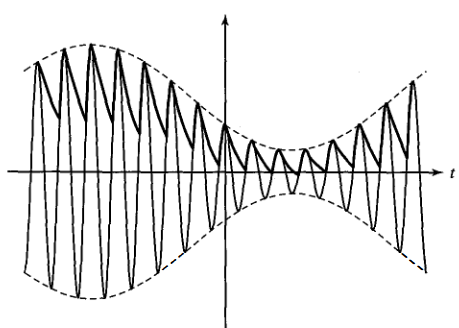
\includegraphics[width= 0.75\textwidth]{Fig/demod_am_conv_baixo_rc.png}  
      \end{center}
    \end{figure}
    
        \begin{block}{Baixa constante RC}
          \begin{itemize}
            \item Saída do filtro varia abruptamente
            \item Presença de compoentes de alta-frequência
          \end{itemize}
        \end{block}        
  \end{column}
  \begin{column}{0.45\textwidth}
    \begin{figure}[!t]
      \begin{center}
        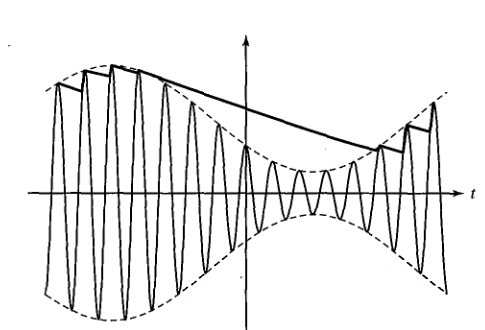
\includegraphics[width= 0.75\textwidth]{Fig/demod_am_conv_alto_rc.png}  
      \end{center}
    \end{figure}
    \begin{block}{Alta constante RC}
          \begin{itemize}
            \item Capacitor demora para carregar
            \item Elimina componentes de alta-frequência da mensagem
          \end{itemize}
    \end{block}        
  \end{column}
\end{columns}
\end{frame}


\section{SSB-AM}

\begin{frame}
  \frametitle{Definição}

   \begin{columns}[T]
    \begin{column}{0.5\textwidth}

      \begin{figure}[!t]
        \begin{center}
          \begin{tikzpicture}
            \begin{axis}[
                width=0.85\textwidth, % Scale the plot to \linewidth
                grid = major, % Display a grid
                grid style={dashed,gray!30}, % Set the style
                xlabel= Frequência, % Set the labels
                ylabel= Amplitude,
                ymin=0, ymax=0.5,
                xmin = -400, xmax = 400,
                x unit=\si{\hertz}, % Set the respective units
                y unit=\si{\volt},
                legend style={at={(0,1.5)},anchor=north west}, % Put the legend below the plot
                %x tick label style={rotate=90,anchor=east} % Display labels sideways
              ]
              
            
              \addplot+ [no marks]
              table[x=Frequencia,y=Amplitude(V)1,col sep=comma] {Fig/sinal_ssb.csv}; 
              
              \addplot+ [no marks,red]
              table[x=Frequencia,y=Amplitude(V)2,col sep=comma] {Fig/sinal_ssb.csv};

              \legend{DSB,SSB}
            \end{axis}
          \end{tikzpicture}
          \caption{Representação em frequênncia do sinal DSB e SSB.}
        \end{center}
      \end{figure}
    \end{column}
    \begin{column}{0.5\textwidth}
      \begin{block}{Características da modulação DSB}
        \begin{itemize}
          \item Espectro simétrico
          \item Canal deve ser no mínimo $2W$
          \item Uso ineficiente do espectro
        \end{itemize}
      \end{block}

      \begin{block}{Características da modulação DSB}
        \begin{itemize}
          \item Requere uma largura de canal de $W$
          \item Considera a simetria do espectro
        \end{itemize}
      \end{block}
    \end{column}


   \end{columns}

  
\end{frame}

\begin{frame}
  \frametitle{Fundamentação para a modulação SSB: Análise na frequência}

  Considere o filtro de transmissão 

$$
H(f) = \begin{cases}
1, & |f| > f_c, \\
0, & \textrm{caso contrário}
\end{cases}
$$

$$
H(f) = U(f - f_c) + U(-f - f_c)
$$

Portanto, o espectro SSB é dado por 

\begin{align*}
  \mathcal{F}[u(t)] & = \mathcal{F}[u_{DSB} \circ h(t)]  \\
                    & = \mathcal{F}[(2Am(t)\cos(2\pi f_ct)) \circ h(t)] \\
                    & = AM(f - f_c)U(f -f_c) + AM(f + f_c)U(-f -f_c) \\
                    & = AM(f)U(f)_{f = f-f_c} + AM(f)U(-f)_{f = f+f_c}
\end{align*}

\end{frame}

\begin{frame}
  \frametitle{Fundamentação para a modulação SSB: Análise no tempo}

  Convertendo para o tempo:


\begin{align*} 
u(t) &= A m(t) \circ  \mathcal{F}^{-1}[U(f)] \exp(\jmath 2 \pi f_c t) + A m(t) \circ  \mathcal{F}^{-1}[U(-f)] \exp(-\jmath 2 \pi f_c t) \\
     &= A m(t) \circ \frac{1}{2}\left( \delta (t) + \frac{\jmath}{2\pi t} \right)\exp(\jmath 2 \pi f_c t) +  A m(t) \circ \frac{1}{2}\left( \delta (t) - \frac{\jmath}{2\pi t} \right)\exp(-\jmath 2 \pi f_c t) \\
     &= \frac{A}{2}[m(t) + \jmath \hat{m}(t)]\exp(\jmath 2 \pi f_c t) + \frac{A}{2}[m(t) - \jmath \hat{m}(t)]\exp(-\jmath 2 \pi f_c t) \\
     &= Am(t)\cos( 2 \pi f_c t) - A\hat{m}(t)\sin( 2 \pi f_c t) 
\end{align*}

Portanto, a expressão banda superior é dada por
$$
u(t) = m(t)\cos( 2 \pi f_c t) - \hat{m}(t)\sin( 2 \pi f_c t).
$$
\end{frame}

\begin{frame}
  \frametitle{}

  Para calcular a banda inferior tem-se que 


\begin{align*}
u(t) + u_l(t) &= 2Am(t)\cos(2\pi f_ct)  \\
u_l(t)        &= 2Am(t)\cos(2\pi f_ct) - A m(t)\cos( 2 \pi f_c t) + A\hat{m}(t)\sin( 2 \pi f_c t) \\
u_l(t)        &= A m(t)\cos( 2 \pi f_c t) + A\hat{m}(t)\sin( 2 \pi f_c t)
\end{align*}

\end{frame}

\section{VSB}
\begin{frame}
  \frametitle{Conceito}


  

\end{frame}


\begin{frame}
  \frametitle{Qual filtro deve ser utilizado?}

  Considere o sinal transmitido

\begin{align*}
 \mathcal{F}[u(t)] & = \mathcal{F}[u_{DSB} \circ h(t)]  \\
                   & = \mathcal{F}[(2Am(t)\cos(2\pi f_ct)) \circ h(t)] \\
                   & = \frac{A}{2}(M(f-f_c) + M(f+f_c))H(f)
\end{align*}

Na entrada do receptor tem-se que :

\begin{align*}
v(t)     &= u(t) \cos(2\pi f_ct)  \\
V(f)     & =\frac{A}{2} [U(f - fc) + U(f + fc)] \\
         &  \frac{A}{4}\left[(M(f-2f_c) + M(f))H(f-f_c) +  (M(f) + M(f+2f_c))H(f+f_c) \right]
\end{align*}

\end{frame}


\begin{frame}
  \frametitle{Qual filtro deve ser utilizado?}

  
Após o uso de filtro passa-baixa

\begin{align*}
V(f)     & =  \frac{A}{4}M(f)\left[(H(f-f_c) + H(f+f_c) \right]
\end{align*}

para que não haja distorção no sinal tem-se que :

$$
H(f-f_c) + H(f+f_c) = \textrm{constante}
$$
\end{frame}


\section{Implementações de moduladores}

\begin{frame}
  \frametitle{Moduladores por série de potência
  }

  Esse tipo de modulador é caracterizado pela a utilização de um dispositivo não-linear. Considere a relação de entrada e saída

$$
v_o(t) = a_1v_i(t) + a_2v_2(t),
$$
em que,
$$
v_i(t) = m(t) +A_c \cos(2\pi f_c t).
$$

O sinal na saída do dispositivo é portanto

\begin {align*}
v_o(t)  &=  a_1m(t) +a_1A_c \cos(2\pi f_c t) + a_2(m^2(t) +A^2_c \cos^2(2\pi f_c t) + 2m(t)A_c \cos^2(2\pi f_c t)) \\
        &=  A_c a_1\left[ 1 + \frac{m(t) a_2}{a_1}\right]\cos(2\pi f_c t) + a_2m^2(t) + a_2A^2_c \cos^2(2\pi f_c t) \\
\end{align*}

\end{frame}


\begin{frame}
  \frametitle{Moduladores por série de potência}

  Após o uso de um filtro de banda-passante o sinal transmitido é 
$$
v_o(t) = A_c a_1\left[ 1 + \frac{m(t) a_2}{a_1}\right]\cos(2\pi f_c t)
$$

\begin{block}{Conclusão}
  Nesta estrutura é possível gerar um sinal AM convecional.
\end{block}

\end{frame}

\section {Exercícios}

\begin{frame}
  \frametitle{Questão 1}

  Considere sistema DSB cuja a portadora é dada por $c(t) = A \cos(2\pi f_c t)$ e a mensagem é $m(t) = \text{sinc}(t) + \text{sinc}(t)^2$. Determine a representação em frequência e a largura de banda do sinal modulado

\end{frame}

\begin{frame}
  \frametitle{Solução}

  Considere 

\begin{align*}
 u(t) &= m(t)c(t) \\
      &=A\left(\text{sinc}(t) + \text{sinc}(t)^2 \right)   \cos(2\pi f_c t) \\
U(f) & = \frac{A}{2} \left[ \Pi (f)  + \Delta (f)\right]  \star  \left(\delta (f-f_c) + \delta (f+f_c) \right) \\
      &= \frac{A}{2} \left[ \Pi (f-f_c)  +  \Delta (f - f_c) +  \Pi (f+f_c)  +  \Delta (f + f_c)\right]
\end{align*}

A função $\Pi (f-f_c) \neq 0$ para $|f-f_c|<1/2$ e  $\Delta (f-f_c) \neq 0$ para $|f-f_c|<1$. Assim, a largura de banda do sinal de banda passante será de 2 Hz


\end{frame}

\begin{frame}
  \frametitle{Questão 2}

  
Considere o sinal $m(t)$
$$
m(t) = 2\cos(4000\pi t) + 5\cos(6000\pi t),
$$
o qual modula a portadora $c(t) = 100\cos(2\pi f_c t)$, em que $f_c = 50$ kHz. Determine and desenhe o espectro do sinal DSB-SC

\end{frame}

\begin{frame}
  \frametitle{Solução}

  Considere $f_1= 2$ kHz e $f_2= 3$ kHz

\begin{align*}
  u(t) & =  2\cos(2\pi f_1 t)\cos(2\pi f_c t) + 5\cos(2\pi f_2 t)\cos(2\pi f_c t)  \text{ Aplicando Fourier ...}  \\ 
  U(f) & = \left[\delta (f - f_1) + \delta (f + f_1) + \frac{5}{2}\delta (f - f_1) + \frac{5}{2}\delta (f + f_1)\right] \star \frac{100
  }{2}\left[ \delta (f - f_c) + \delta (f + f_c)\right] \\
     & =  \frac{100}{2}\left[\delta (f - f_1 - fc)  + \delta (f + f_1 - fc) + \frac{5}{2}\delta (f - f_1 - fc) + \frac{5}{2}\delta (f + f_1 - fc)\right] + \\
     & \frac{100}{2}\left[\delta (f - f_1 + fc)  + \delta (f + f_1 + fc) + \frac{5}{2}\delta (f - f_1 + fc) + \frac{5}{2}\delta (f + f_1 + fc)\right] 
\end{align*}

Portanto as componentes de frequência serão 


\begin{itemize}
  \item  $f_c - f_1 = 50  - 2 = 48$ \si{\kilo\hertz} 
  \item $f_c - f_2 = 50  - 3 = 47$ \si{\kilo\hertz} 
  \item $f_c + f_1 = 50  + 2 = 52$ \si{\kilo\hertz} 
  \item $f_c + f_2 = 50  + 4 = 53$ \si{\kilo\hertz}
  
\end{itemize}

\end{frame}
\end{document}